\documentclass[12pt]{article}
\usepackage[margin=0.7in]{geometry}
\usepackage{graphicx}
\usepackage{amsmath}
\usepackage{float}
\usepackage{capt-of}
\usepackage{varwidth}
\usepackage{booktabs}

% Define a command to layout a table
% Inpute values are #1 input layer bias node
%                   #2 hidden layer bias node
%                   #3 standardization of features
%                   #4 PCA applied
%                   #5 LDA applied
%                   #6 Accuracy
%                   #7 Testing Error
%                   #8 Table Caption
\newcommand{\accuracyAndTestErrorTable}[8]{
  \begin{tabular}{l|l}
    \hline
    Input layer bias node & #1 \\
    Hidden layer bias node & #2 \\
    Standardization of features & #3 \\
    PCA applied & #4 \\
    LDA applied & #5 \\
    \hline
    Testing Accuracy & #6 \\
    Testing Error & #7 \\
    \hline
  \end{tabular}
  ~\\[60pt]
  \caption{#8}
}

\begin{document}

\begin{titlepage}

\newcommand{\HRule}{\rule{\linewidth}{0.5mm}} % Defines a new command for the horizontal lines, change thickness here

\center % Center everything on the page

%----------------------------------------------------------------------------------------
%	HEADING SECTIONS
%----------------------------------------------------------------------------------------

\textsc{\LARGE Drexel University}\\[1.5cm] % Name of your university/college
\textsc{\Large CS499I}\\[0.5cm] % Major heading such as course name
\textsc{\large Advanced Neural Networks}\\[0.5cm] % Minor heading such as course title

%----------------------------------------------------------------------------------------
%	TITLE SECTION
%----------------------------------------------------------------------------------------

\HRule \\[0.4cm]
{ \huge \bfseries Facial Recognition With Artificial Neural Networks}\\[0.4cm] % Title of your document
\HRule \\[1.5cm]

%----------------------------------------------------------------------------------------
%	AUTHOR SECTION
%----------------------------------------------------------------------------------------

\begin{minipage}{0.4\textwidth}
\begin{flushleft} \large
\emph{Author:}\\
Alexander \textsc{Marion}\\
Matthew \textsc{D'Amore}
\end{flushleft}
\end{minipage}
~
\begin{minipage}{0.4\textwidth}
\begin{flushright} \large
\emph{Supervisor:} \\
Dr. Matthew \textsc{Burlick}
\end{flushright}
\end{minipage}\\[4cm]

% If you don't want a supervisor, uncomment the two lines below and remove the section above
%\Large \emph{Author:}\\
%John \textsc{Smith}\\[3cm] % Your name

%----------------------------------------------------------------------------------------
%	DATE SECTION
%----------------------------------------------------------------------------------------

{\large \today}\\[3cm] % Date, change the \today to a set date if you want to be precise

%----------------------------------------------------------------------------------------
%	LOGO SECTION
%----------------------------------------------------------------------------------------

%\includegraphics{Logo}\\[1cm] % Include a department/university logo - this will require the graphicx package

%----------------------------------------------------------------------------------------

\vfill % Fill the rest of the page with whitespace
\end{titlepage}

\newpage

\section{Datasets}
\textbf{Yale Faces Database} \quad This dataset contains 165 grayscale images in GIF format of 15 individuals with 11 images per person. There is one image per each of the following configurations: center-light, w/glasses, happy, left-light, w/no glasses, normal, right-light, sad, sleepy, surprised, and wink.

\section{Testing Parameters}
The following variants are tested for accuracy:
\begin{enumerate}
  \item With and without a bias node at the input layer
  \item With and without a bias node at the hidden layer
  \item With and without standardizing features
  \item With and without applying PCA to reduce the number of features to 95\%
  \item With and without applying LDA to maximize data separability
\end{enumerate}
Empirical data was generated to optimize the following parameters:
\begin{enumerate}
  \item Image size
  \item Hidden layer size
  \item Termination criteria
\end{enumerate}

\section{Baseline Accuracy}
The baseline accuracy was created using the negative form of all variants with the exception of data standardization. The baseline parameters were as follows: 40 by 40 sized images, a hidden layer size of 20, and 1000 training iterations.
\begin{center}
  \begin{table}[H]
    \begin{varwidth}[b]{0.4\linewidth}
      \centering
      \accuracyAndTestErrorTable{N}{N}{Y}{N}{N}{0.800000}{0.200000}{Baseline accuracy and testing}
      \label{table:baseline}
    \end{varwidth}%
    \hfill
    \begin{minipage}[b]{0.6\linewidth}
      \centering
      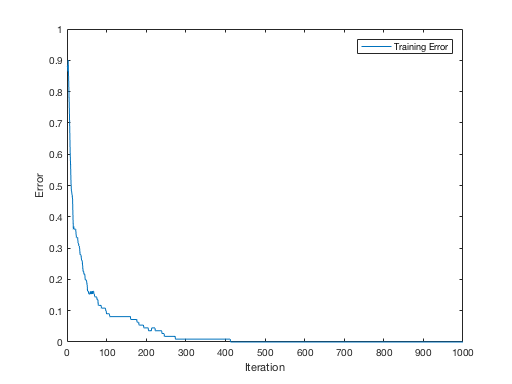
\includegraphics[width=100mm]{baseline_training_error.png}
      \captionof{figure}{Plot of baseline training error}
      \label{fig:baseline_img}
    \end{minipage}
  \end{table}
\end{center}

% NNNNN
\section{Variant Accuracy Testing}
All variants were tested using 40 by 40 sized images, a hidden layer size of 20, and 1000 training iterations.
\begin{center}
  \begin{table}[H]
    \begin{varwidth}[b]{0.4\linewidth}
      \centering
      \accuracyAndTestErrorTable{N}{N}{N}{N}{N}{0.145455}{0.854545}{NNNNN accuracy and testing}
      \label{table:NNNNN}
    \end{varwidth}%
    \hfill
    \begin{minipage}[b]{0.6\linewidth}
      \centering
      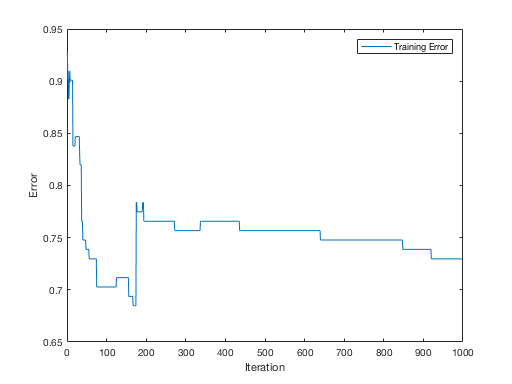
\includegraphics[width=100mm]{NNNNN_training_error.png}
      \captionof{figure}{Plot of NNNNN training error}
      \label{fig:NNNNN}
    \end{minipage}
  \end{table}
\end{center}

% YNNNN
\begin{center}
  \begin{table}[H]
    \begin{varwidth}[b]{0.4\linewidth}
      \centering
      \accuracyAndTestErrorTable{Y}{N}{N}{N}{N}{0.272727}{0.727273}{YNNNN accuracy and testing}
      \label{table:YNNNN}
    \end{varwidth}%
    \hfill
    \begin{minipage}[b]{0.6\linewidth}
      \centering
      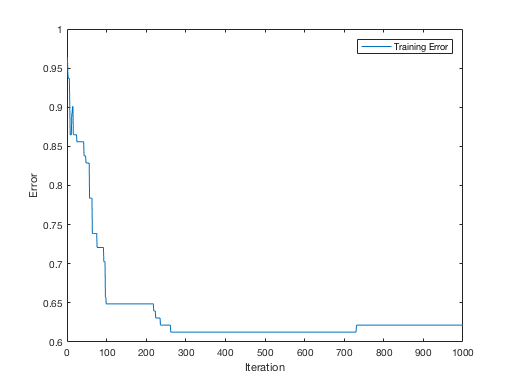
\includegraphics[width=100mm]{YNNNN_training_error.png}
      \captionof{figure}{Plot of YNNNN training error}
      \label{fig:YNNNN}
    \end{minipage}
  \end{table}
\end{center}


% NYNNN
\begin{center}
  \begin{table}[H]
    \begin{varwidth}[b]{0.4\linewidth}
      \centering
      \accuracyAndTestErrorTable{N}{Y}{N}{N}{N}{0.181818}{0.818182}{NYNNN accuracy and testing}
      \label{table:NYNNN}
    \end{varwidth}%
    \hfill
    \begin{minipage}[b]{0.6\linewidth}
      \centering
      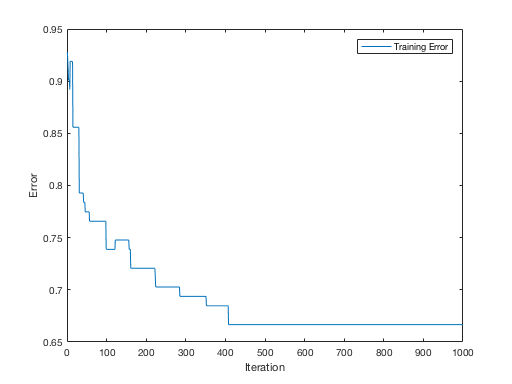
\includegraphics[width=100mm]{NYNNN_training_error.png}
      \captionof{figure}{Plot of NYNNN training error}
      \label{fig:NYNNN}
    \end{minipage}
  \end{table}
\end{center}

% NNNYN
\begin{center}
  \begin{table}[H]
    \begin{varwidth}[b]{0.4\linewidth}
      \centering
      \accuracyAndTestErrorTable{N}{N}{N}{Y}{N}{0.254545}{0.745455}{NNNYN accuracy and testing}
      \label{table:NNNYN}
    \end{varwidth}%
    \hfill
    \begin{minipage}[b]{0.6\linewidth}
      \centering
      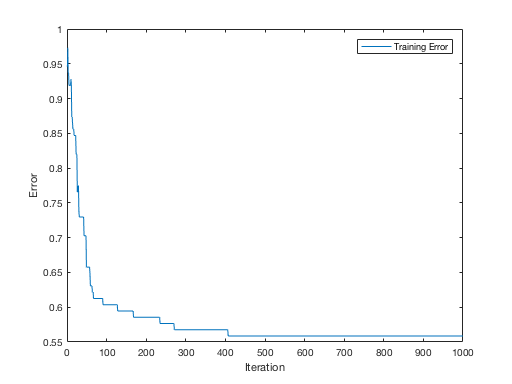
\includegraphics[width=100mm]{NNNYN_training_error.png}
      \captionof{figure}{Plot of NNNYN training error}
      \label{fig:NNNYN}
    \end{minipage}
  \end{table}
\end{center}



% NNNNY



% YYNNN
\begin{center}
  \begin{table}[H]
    \begin{varwidth}[b]{0.4\linewidth}
      \centering
      \accuracyAndTestErrorTable{Y}{Y}{N}{N}{N}{0.400000}{0.600000}{YYNNN accuracy and testing}
      \label{table:YYNNN}
    \end{varwidth}%
    \hfill
    \begin{minipage}[b]{0.6\linewidth}
      \centering
      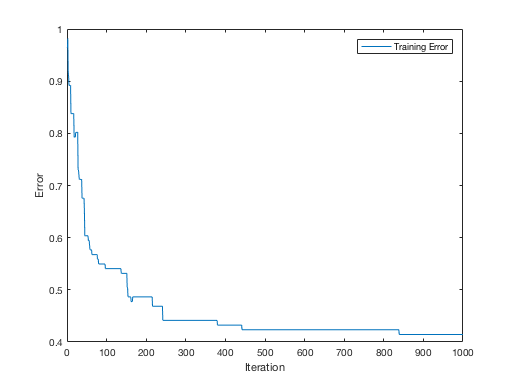
\includegraphics[width=100mm]{YYNNN_training_error.png}
      \captionof{figure}{Plot of YYNNN training error}
      \label{fig:YYNNN}
    \end{minipage}
  \end{table}
\end{center}

% YNYNN
\begin{center}
  \begin{table}[H]
    \begin{varwidth}[b]{0.4\linewidth}
      \centering
      \accuracyAndTestErrorTable{Y}{N}{Y}{N}{N}{0.818182}{0.181818}{YNYNN accuracy and testing}
      \label{table:YNYNN}
    \end{varwidth}%
    \hfill
    \begin{minipage}[b]{0.6\linewidth}
      \centering
      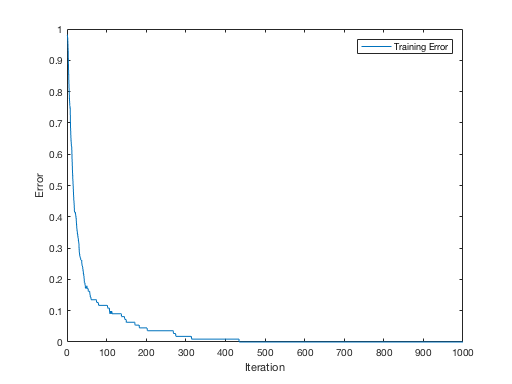
\includegraphics[width=100mm]{YNYNN_training_error.png}
      \captionof{figure}{Plot of YNYNN training error}
      \label{fig:YNYNN}
    \end{minipage}
  \end{table}
\end{center}

% YNNYN
\begin{center}
  \begin{table}[H]
    \begin{varwidth}[b]{0.4\linewidth}
      \centering
      \accuracyAndTestErrorTable{Y}{N}{N}{Y}{N}{0.200000}{0.800000}{YNNYN accuracy and testing}
      \label{table:YNNYN}
    \end{varwidth}%
    \hfill
    \begin{minipage}[b]{0.6\linewidth}
      \centering
      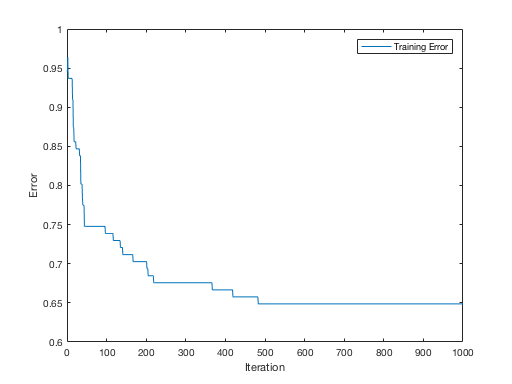
\includegraphics[width=100mm]{YNNYN_training_error.png}
      \captionof{figure}{Plot of YNNYN training error}
      \label{fig:YNNYN}
    \end{minipage}
  \end{table}
\end{center}


% YNNNY


% NYYNN
\begin{center}
  \begin{table}[H]
    \begin{varwidth}[b]{0.4\linewidth}
      \centering
      \accuracyAndTestErrorTable{N}{Y}{Y}{N}{N}{0.818182}{0.181818}{NYYNN accuracy and testing}
      \label{table:NYYNN}
    \end{varwidth}%
    \hfill
    \begin{minipage}[b]{0.6\linewidth}
      \centering
      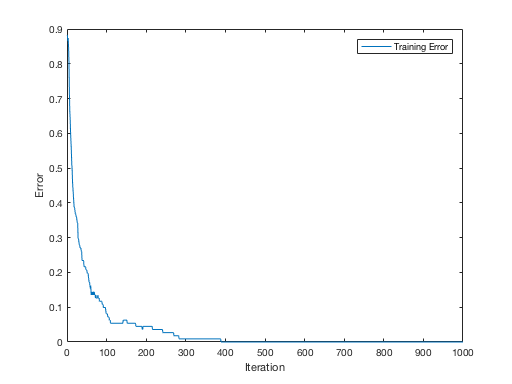
\includegraphics[width=100mm]{NYYNN_training_error.png}
      \captionof{figure}{Plot of NYYNN training error}
      \label{fig:NYYNN}
    \end{minipage}
  \end{table}
\end{center}

% NYNYN
\begin{center}
  \begin{table}[H]
    \begin{varwidth}[b]{0.4\linewidth}
      \centering
      \accuracyAndTestErrorTable{N}{Y}{N}{Y}{N}{0.254545}{0.745455}{NYNYN accuracy and testing}
      \label{table:NYNYN}
    \end{varwidth}%
    \hfill
    \begin{minipage}[b]{0.6\linewidth}
      \centering
      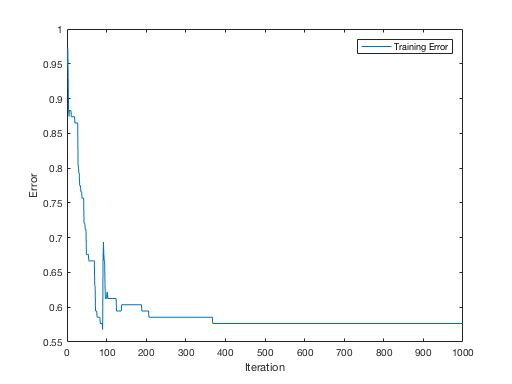
\includegraphics[width=100mm]{NYNYN_training_error.png}
      \captionof{figure}{Plot of NYNYN training error}
      \label{fig:NYNYN}
    \end{minipage}
  \end{table}
\end{center}


% NYNNY


% NNYYN
\begin{center}
  \begin{table}[H]
    \begin{varwidth}[b]{0.4\linewidth}
      \centering
      \accuracyAndTestErrorTable{N}{N}{Y}{Y}{N}{0.145455}{0.854545}{NNYYN accuracy and testing}
      \label{table:NNYYN}
    \end{varwidth}%
    \hfill
    \begin{minipage}[b]{0.6\linewidth}
      \centering
      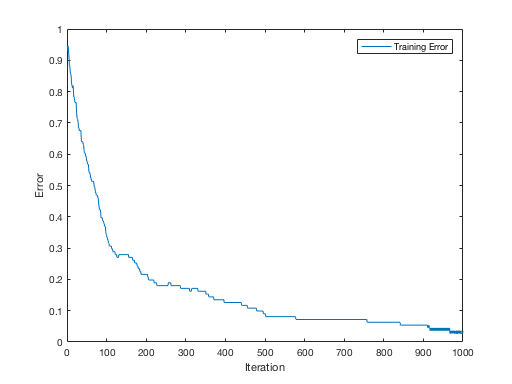
\includegraphics[width=100mm]{NNYYN_training_error.png}
      \captionof{figure}{Plot of NNYYN training error}
      \label{fig:NNYYN}
    \end{minipage}
  \end{table}
\end{center}


% NNYNY


% YYYNN
\begin{center}
  \begin{table}[H]
    \begin{varwidth}[b]{0.4\linewidth}
      \centering
      \accuracyAndTestErrorTable{Y}{Y}{Y}{N}{N}{0.800000}{0.200000}{YYYNN accuracy and testing}
      \label{table:YYYNN}
    \end{varwidth}%
    \hfill
    \begin{minipage}[b]{0.6\linewidth}
      \centering
      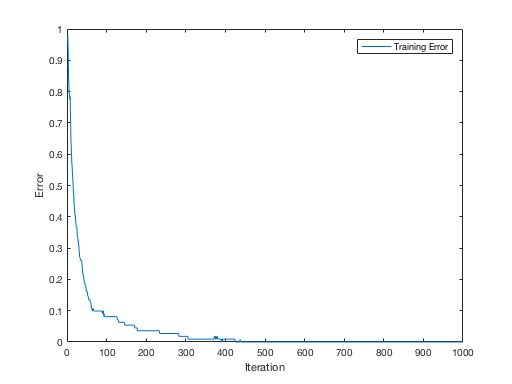
\includegraphics[width=100mm]{YYYNN_training_error.png}
      \captionof{figure}{Plot of YYYNN training error}
      \label{fig:YYYNN}
    \end{minipage}
  \end{table}
\end{center}

% YYNYN
\begin{center}
  \begin{table}[H]
    \begin{varwidth}[b]{0.4\linewidth}
      \centering
      \accuracyAndTestErrorTable{Y}{Y}{N}{Y}{N}{0.200000}{0.800000}{YYNYN accuracy and testing}
      \label{table:YYNYN}
    \end{varwidth}%
    \hfill
    \begin{minipage}[b]{0.6\linewidth}
      \centering
      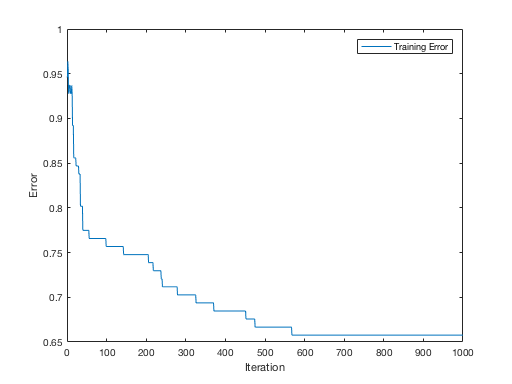
\includegraphics[width=100mm]{YYNYN_training_error.png}
      \captionof{figure}{Plot of YYNYN training error}
      \label{fig:YYNYN}
    \end{minipage}
  \end{table}
\end{center}


% YYNNY


% YNYYN
\begin{center}
  \begin{table}[H]
    \begin{varwidth}[b]{0.4\linewidth}
      \centering
      \accuracyAndTestErrorTable{Y}{N}{Y}{Y}{N}{0.181818}{0.818182}{YNYYN accuracy and testing}
      \label{table:YNYYN}
    \end{varwidth}%
    \hfill
    \begin{minipage}[b]{0.6\linewidth}
      \centering
      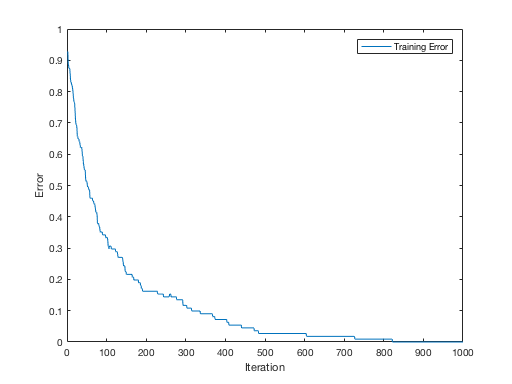
\includegraphics[width=100mm]{YNYYN_training_error.png}
      \captionof{figure}{Plot of YNYYN training error}
      \label{fig:YNYYN}
    \end{minipage}
  \end{table}
\end{center}


% YNYNY


% NYYYN
\begin{center}
  \begin{table}[H]
    \begin{varwidth}[b]{0.4\linewidth}
      \centering
      \accuracyAndTestErrorTable{N}{Y}{Y}{Y}{N}{0.145455}{0.854545}{NYYYN accuracy and testing}
      \label{table:NYYYN}
    \end{varwidth}%
    \hfill
    \begin{minipage}[b]{0.6\linewidth}
      \centering
      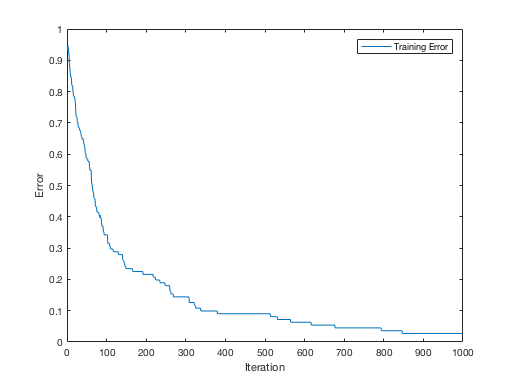
\includegraphics[width=100mm]{NYYYN_training_error.png}
      \captionof{figure}{Plot of NYYYN training error}
      \label{fig:NYYYN}
    \end{minipage}
  \end{table}
\end{center}


% NYYNY


% YYYYN
\begin{center}
  \begin{table}[H]
    \begin{varwidth}[b]{0.4\linewidth}
      \centering
      \accuracyAndTestErrorTable{Y}{Y}{Y}{Y}{N}{0.181818}{0.818182}{YYYYN accuracy and testing}
      \label{table:YYYYN}
    \end{varwidth}%
    \hfill
    \begin{minipage}[b]{0.6\linewidth}
      \centering
      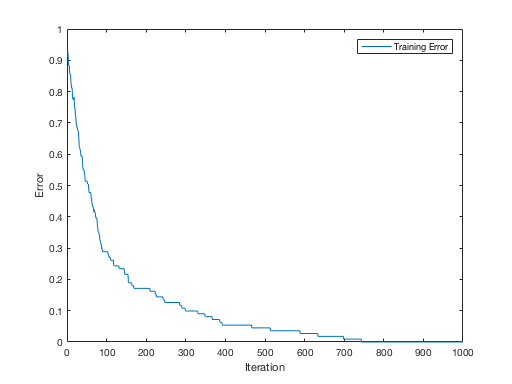
\includegraphics[width=100mm]{YYYYN_training_error.png}
      \captionof{figure}{Plot of YYYYN training error}
      \label{fig:YYYYN}
    \end{minipage}
  \end{table}
\end{center}

% YYYNY

\section{Empirical Parameter Accuracy Testing}
All empirical data was gathered using the following variant which had the highest accuracy from the variant testing:
\begin{center}
  \begin{table}[H]
    \begin{varwidth}[b]{0.4\linewidth}
      \centering
      \accuracyAndTestErrorTable{Y}{N}{Y}{N}{N}{0.818182}{0.181818}{YNYNN accuracy and testing}
      \label{table:param_base}
    \end{varwidth}%
    \hfill
    \begin{minipage}[b]{0.6\linewidth}
      \centering
      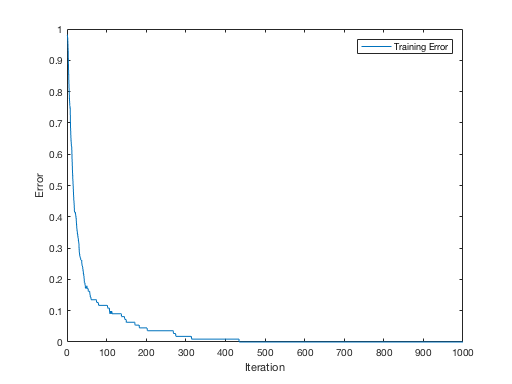
\includegraphics[width=100mm]{YNYNN_training_error.png}
      \captionof{figure}{Plot of YNYNN training error}
      \label{fig:param_base}
    \end{minipage}
  \end{table}
\end{center}

\begin{enumerate}
  \item Number of Training Iterations
  The number of training iterations was varied from 0 to 10,000 by 100. The number of hidden nodes was 20 and the image size was 40 by 40. The following is a plot of the accuracy as number of training iterations increases.
  \begin{center}
    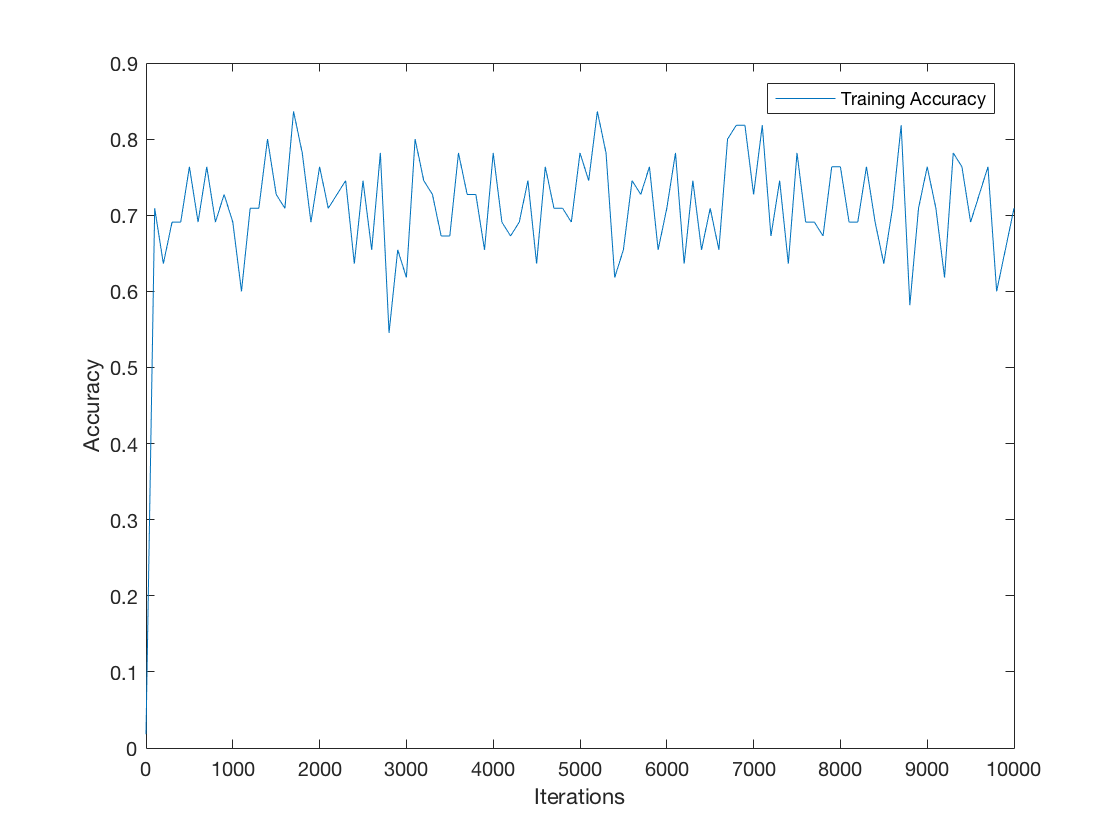
\includegraphics[width=125mm]{num_iterations_empirical.png}
    \captionof{figure}{Plot of accuracy as number of training iterations increases}
    \label{fig:num_iterations}
  \end{center}
  \item Number of Hidden Nodes
  The number of hidden nodes was varied from 0 to 1600 (the number of features) by 20. The number of training iterations was 1000 and the image size was 40 by 40. The following is a plot of the accuracy as number of hidden nodes increases.
  \begin{center}
    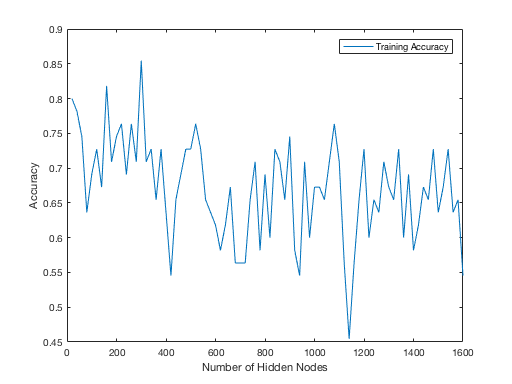
\includegraphics[width=125mm]{hidden_node_empirical.png}
    \captionof{figure}{Plot of accuracy as number of hidden nodes increases}
    \label{fig:num_hidden_nodes}
  \end{center}
  \item Image Size
\end{enumerate}


\end{document}
